\documentclass[conference]{IEEEtran}
\IEEEoverridecommandlockouts
% The preceding line is only needed to identify funding in the first footnote. If that is unneeded, please comment it out.
\usepackage{cite}
\usepackage{amsmath,amssymb,amsfonts}
\usepackage{algorithmic}
\usepackage{graphicx}
\usepackage{textcomp}
\usepackage{xcolor}
\usepackage{hyperref}
\def\BibTeX{{\rm B\kern-.05em{\sc i\kern-.025em b}\kern-.08em
    T\kern-.1667em\lower.7ex\hbox{E}\kern-.125emX}}
\begin{document}

\title{COSC325 Project Proposal}

\author{\IEEEauthorblockN{Stefan Smith}
ssmit493@vols.utk.edu
\and
\IEEEauthorblockN{Dennis Madapatu}
netid@vols.utk.edu
\and
\IEEEauthorblockN{Matthew Ferrari}
dwp393@vols.utk.edu
\and
\IEEEauthorblockN{Faraz Ghouri}
netid@vols.utk.edu
\and
\IEEEauthorblockN{Alex Worthington}
netid@vols.utk.edu
\and
\IEEEauthorblockN{Bam Adebayo}
bammy@miamiheat.com

}

\maketitle

\section{Problem and Motivation}
% Problem & motivation: What are you solving and why? Which dataset and why is it appropriate?
Here, we propose our final project for COSC325 - Introduction to Machine Learning. We shall use various machine learning methods - such as linear regression, decision trees, and random forest - to predict housing prices based on a collection of features. Our goal is to understand the benefits and drawbacks of different machine learning models first hand.

We are using the the \href{https://www.kaggle.com/competitions/house-prices-advanced-regression-techniques/data}{"House Prices - Advanced Regression Techniques"} from Kaggle. This data set is appropriate because it has a large set of features and samples - much higher than any other data set we've used in class or in our homework assignments. This way, we will can also practice feature selection and extraction where it might be practical. 

\section{Dataset and EDA}

Dataset and EDA (need 1 -2 people to work on this) : Show your data — distributions, class balance, missing values, 2–3 visualizations. Most important part. Find data that correlates, what features are more important than others

The data used is an advanced housing dataset sourced from kaggle. In this dataset we use log transformation to normalize the distribution \ref{fig:norm}, compressing the range of high value outliers and expanding the range of lower values. This step is important for linear regression models.
\begin{figure}[h]
    \centering
    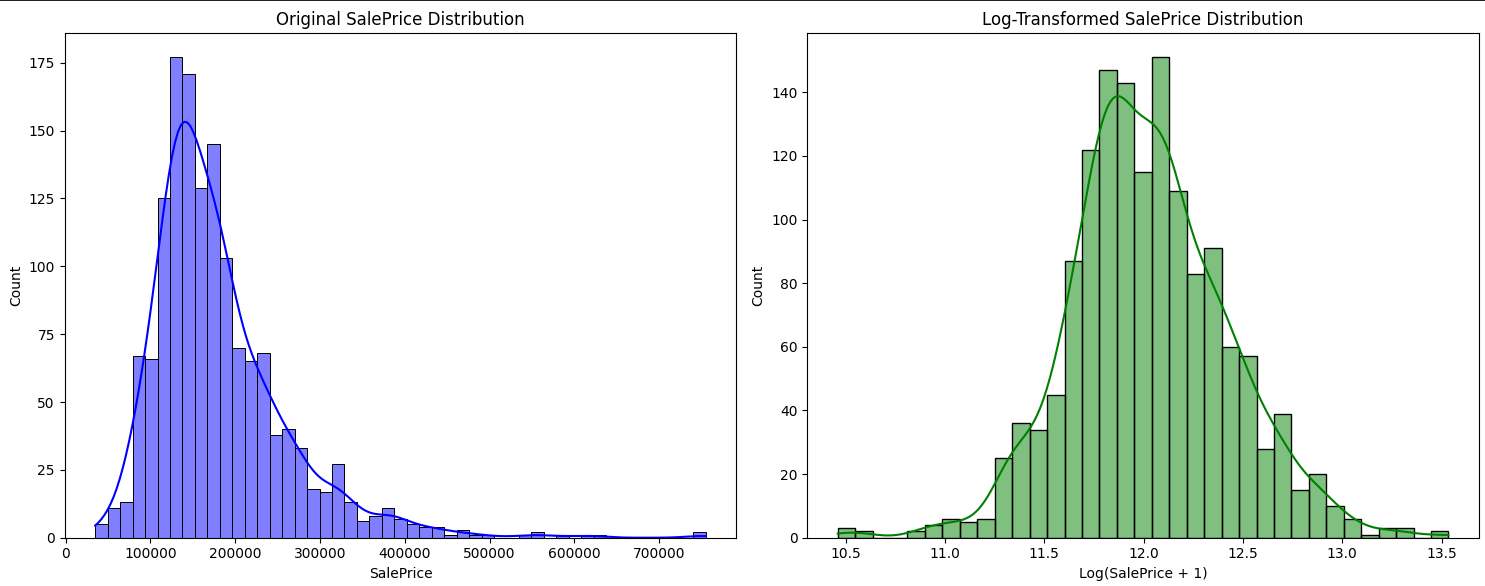
\includegraphics[width=0.2\textwidth]{Normalization.png}
    \caption{Normalization of SalePrice}
    \label{fig:norm}
\end{figure}

\subsection{Class Balance}

The majority of houses are priced between \$100k and \$250k, \ref{fig:balance} with fewer samples below and above this range. This can cause prediction for houses less than \$\$ 1000 and greater than \$300k to be less reliable. 
\begin{figure}[h]
    \centering
    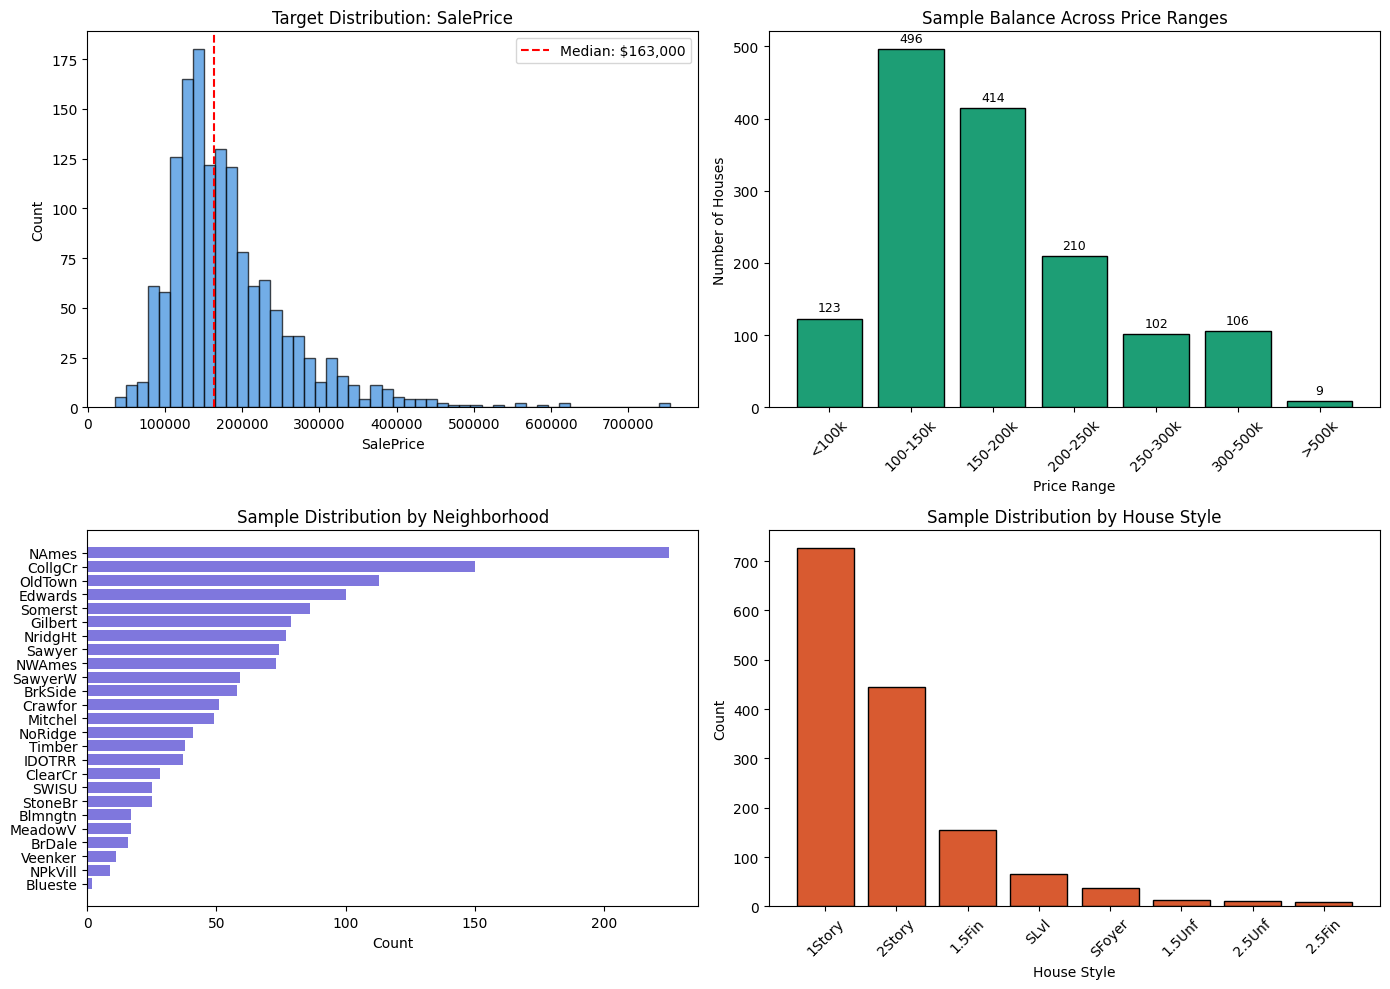
\includegraphics[width=0.2\textwidth]{balance.png}
    \caption{Class Balance of house Sale Price}
    \label{fig:balance}
\end{figure}

\subsection{Missing Values}

For missing data, features that indicate absence, valued ''NaN'' in features: ''PoolQC'', ''Fence'', etc... we fill these with ''None'' to distibguish houses with and without these features. We use context for other features such as ''LotFrontage'' by entering the median Frontage of the dataset. 


\subsection{Feature Correlation}
From Figure ~\ref{fig:correlation}
From graph 3, we can see the top 10 most important features. OverallQual, measurements like square footage, and the newness of the house being built are features that are most correlated with SalesPrice. This is obvious, but this is shown through the training process in which data is trended to see with features have stronger and weaker linear trend with housing price. This can be see in feature 4. 
\begin{figure}[h]
    \centering
    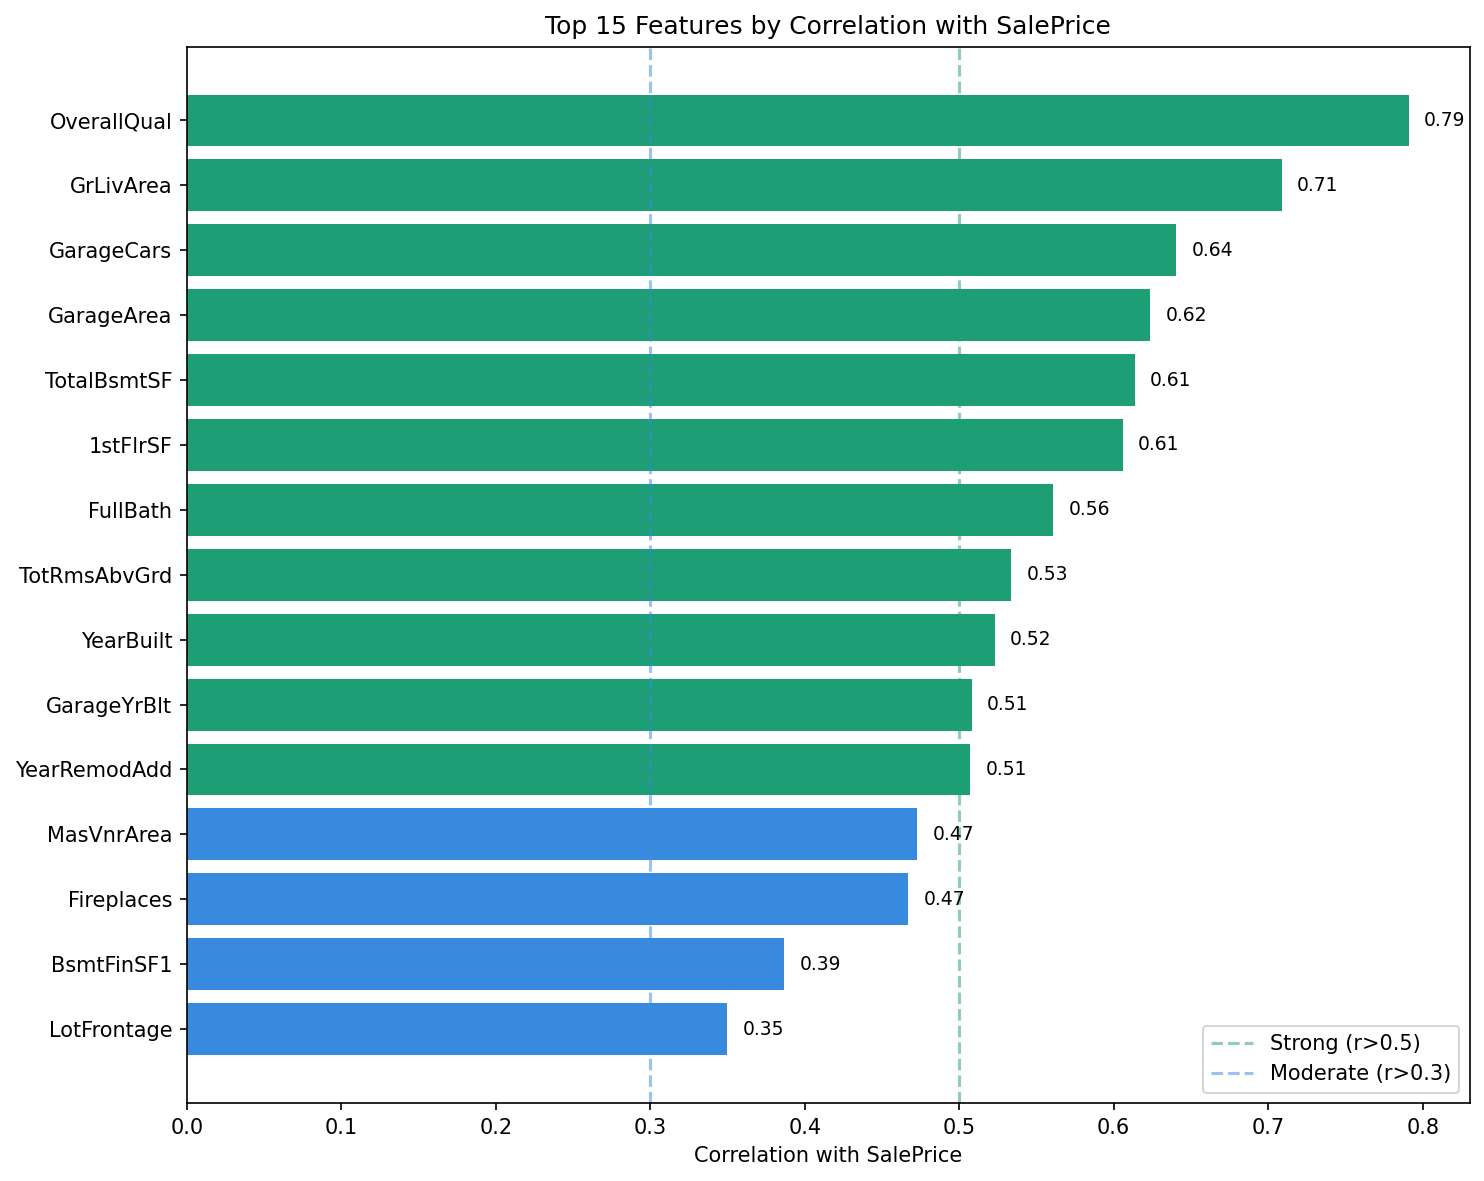
\includegraphics[width=0.2\textwidth]{correlation_ranking.png}
    \caption{Top 10 features most correlated with SalePrice. OverallQual shows the strongest correlation (r=0.79), followed by GrLivArea (r=0.71).}
    \label{fig:correlation}
\end{figure}

\section{Proposed Approach}

Proposed approach: (2-3 people) (try multiple models) : Which models will you try and why? What evaluation metric fits your problem? No implementation needed yet.

\section{Team Roles}

Who is doing what? Data, modelling, writing, coordination. Be specific.

\section*{References}

Please number citations consecutively within brackets \cite{b1}. The 
sentence punctuation follows the bracket \cite{b2}. Refer simply to the reference 
number, as in \cite{b3}---do not use ``Ref. \cite{b3}'' or ``reference \cite{b3}'' except at 
the beginning of a sentence: ``Reference \cite{b3} was the first $\ldots$''

Number footnotes separately in superscripts. Place the actual footnote at 
the bottom of the column in which it was cited. Do not put footnotes in the 
abstract or reference list. Use letters for table footnotes.

Unless there are six authors or more give all authors' names; do not use 
``et al.''. Papers that have not been published, even if they have been 
submitted for publication, should be cited as ``unpublished'' \cite{b4}. Papers 
that have been accepted for publication should be cited as ``in press'' \cite{b5}. 
Capitalize only the first word in a paper title, except for proper nouns and 
element symbols.

For papers published in translation journals, please give the English 
citation first, followed by the original foreign-language citation \cite{b6}.

\end{document}

COSC325-Midterm-Report.tex
4 KB
traxyy — 30 Mar 2026 20:35
I'm Faraz
Professor isn't the worst, I'm just not that interested in ML tbh 
traxyy — 30 Mar 2026 20:50
Since it only needs to be one file, do u want to make a github rep with this? Or do u just want us to send u details about us and u fill it in?
stefs — 30 Mar 2026 21:04
Honestly let’s just answer the questions here and I can paste them into the document
traxyy — 30 Mar 2026 21:04
Sure I dont mind but for project we're gonna have to come up w something else so we can all work together
my netID is fghouri@ -> Faraz Ghouri
stefs — 30 Mar 2026 21:05
Yeah we need to figure out project roles, I can write it out once we do
traxyy — 30 Mar 2026 21:05
Fs 
I'm gonna get started on Step #2
rari — 30 Mar 2026 21:07
I'm gonna start on my part or whatever is next tomorrow. I've gotta lock down my writing for an in class essay tmrw.
alex — 30 Mar 2026 21:13
my netid is aworthi4

\documentclass[conference]{IEEEtran}
\IEEEoverridecommandlockouts
% The preceding line is only needed to identify funding in the first footnote. If that is unneeded, please comment it out.
\usepackage{cite}
\usepackage{amsmath,amssymb,amsfonts}
\usepackage{algorithmic}
\usepackage{graphicx}
\usepackage{textcomp}
\usepackage{xcolor}
\usepackage{hyperref}
\def\BibTeX{{\rm B\kern-.05em{\sc i\kern-.025em b}\kern-.08em
    T\kern-.1667em\lower.7ex\hbox{E}\kern-.125emX}}
\begin{document}

\title{COSC325 Project Proposal}

\author{\IEEEauthorblockN{Stefan Smith}
ssmit493@vols.utk.edu
\and
\IEEEauthorblockN{Dennis Madapatu}
netid@vols.utk.edu
\and
\IEEEauthorblockN{Matthew Ferrari}
netid@vols.utk.edu
\and
\IEEEauthorblockN{Faraz Ghouri}
netid@vols.utk.edu
\and
\IEEEauthorblockN{Alex Worthington}
netid@vols.utk.edu
\and
\IEEEauthorblockN{Bam Adebayo}
bammy@miamiheat.com

}

\maketitle

\section{Problem and Motivation}
% Problem & motivation: What are you solving and why? Which dataset and why is it appropriate?
Here, we propose our final project for COSC325 - Introduction to Machine Learning. We shall use various machine learning methods - such as linear regression, decision trees, and random forest - to predict housing prices based on a collection of features. Our goal is to understand the benefits and drawbacks of different machine learning models first hand.

We are using the the \href{https://www.kaggle.com/competitions/house-prices-advanced-regression-techniques/data}{"House Prices - Advanced Regression Techniques"} from Kaggle. This data set is appropriate because it has a large set of features and samples - much higher than any other data set we've used in class or in our homework assignments. This way, we will can also practice feature selection and extraction where it might be practical. 

\section{Dataset and EDA}

Dataset and EDA (need 1 -2 people to work on this) : Show your data — distributions, class balance, missing values, 2–3 visualizations. Most important part. Find data that correlates, what features are more important than others

\section{Proposed Approach}

Proposed approach: (2-3 people) (try multiple models) : Which models will you try and why? What evaluation metric fits your problem? No implementation needed yet.

\section{Team Roles}

Who is doing what? Data, modelling, writing, coordination. Be specific.

\section*{References}

Please number citations consecutively within brackets \cite{b1}. The 
sentence punctuation follows the bracket \cite{b2}. Refer simply to the reference 
number, as in \cite{b3}---do not use ``Ref. \cite{b3}'' or ``reference \cite{b3}'' except at 
the beginning of a sentence: ``Reference \cite{b3} was the first $\ldots$''

Number footnotes separately in superscripts. Place the actual footnote at 
the bottom of the column in which it was cited. Do not put footnotes in the 
abstract or reference list. Use letters for table footnotes.

Unless there are six authors or more give all authors' names; do not use 
``et al.''. Papers that have not been published, even if they have been 
submitted for publication, should be cited as ``unpublished'' \cite{b4}. Papers 
that have been accepted for publication should be cited as ``in press'' \cite{b5}. 
Capitalize only the first word in a paper title, except for proper nouns and 
element symbols.

For papers published in translation journals, please give the English 
citation first, followed by the original foreign-language citation \cite{b6}.

\end{document}
COSC325-Midterm-Report.tex
4 KB